\section{Forschungsarbeit und Arbeitsprogramm}
\label{sec:4}
%\textit{Beschreibung der geplanten Forschungsarbeiten und des Arbeitsprogramms, unter Einschluss der Darstellung von Methoden, die zur Anwendung kommen bzw. entwickelt werden sollen; sowie der disziplinären Zusammensetzung der geplanten Nachwuchsgruppe}\\
%\textit{FRAGE: Methoden, Disziplinen als Unterpunkte?}\\

\begin{figure}[!h]
    \centering
    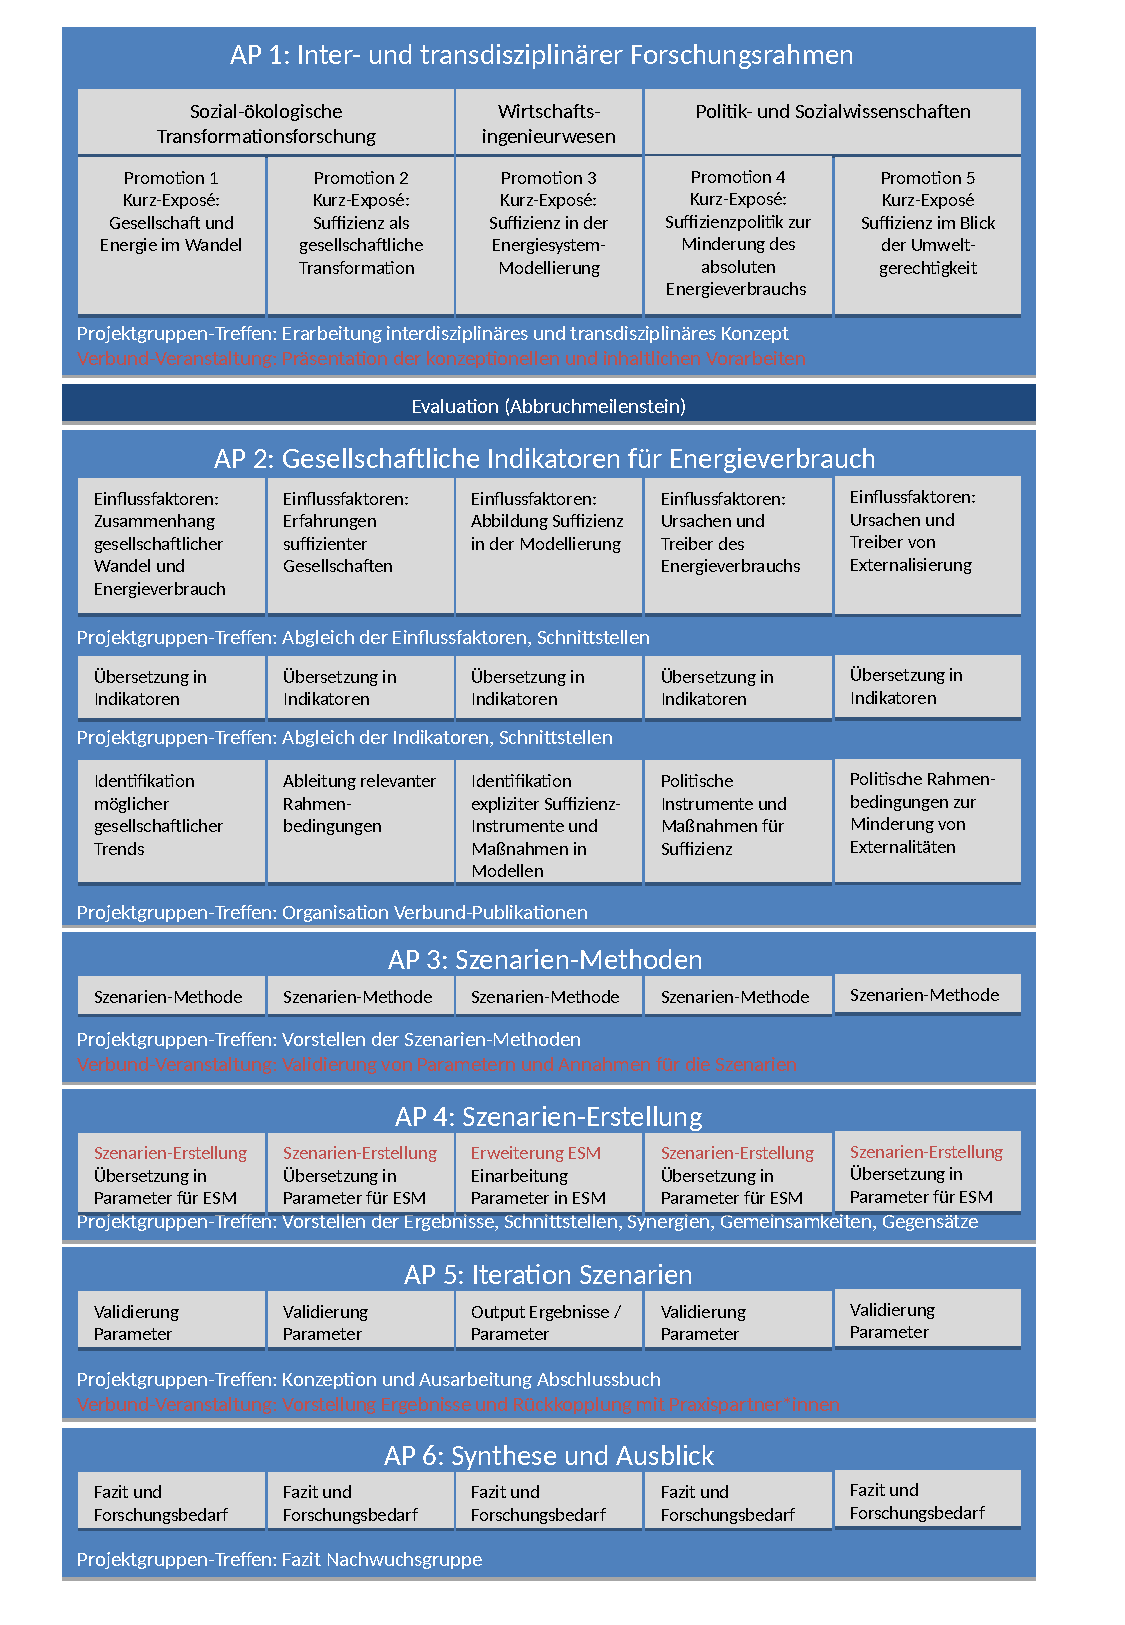
\includegraphics[width=0.9\textwidth]{figures/Forschungsarbeit2.pdf}
    \caption{Das Forschungsprogramm der Nachwuchsforschungsgruppe setzt sich aus sechs interdisziplinären Arbeitspaketen zusammen, in denen die Forschungs-Schwerpunkte der fünf  Promotionsvorhaben (vertikal dargestellt) eingebettet sind}
    \label{fig:forschungsprogramm}
\end{figure}

Abbildung \ref{fig:forschungsprogramm} skizziert die fünf Promotionsvorhaben (vertikal dargestellt) in drei Forschungs-Schwerpunkten, die über die sechs interdisziplinären Arbeitspakete (horizontal dargestellt) ineinander greifen. Im Folgenden wird jeder Forschungs-Schwerpunkt sowie die interdisziplinären Arbeitspakete kurz erläutert.

\subsection*{Forschungs-Schwerpunkt sozial-ökologische Transformationsforschung: Gesellschaftlicher Wandel und Energieverbrauch}

Vergangene umfassende gesellschaftliche Transformationen sind immer mit einer Veränderung der energetischen Basis von Gesellschaften einher gegangen, dies ist in der sozial-ökologischen Forschung verschiedentlich herausgearbeitet worden. Die am NEC angesiedelten Promotionen folgen dieser Erkenntnis insofern, als in einer Arbeit in historischer Perspektive Zusammenhänge zwischen Energieverbrauch und sozialem Wandel insbesondere seit den 1950er Jahren herausgearbeitet werden. Die zweite Arbeit ist dem Blick in wahrscheinliche, mögliche und wünschbare Zukünfte (Kreibich 2008) und der Frage gewidmet, wie gesellschaftliche Veränderungen und Trends künftig mit Energieverfügbarkeit und -nachfrage interagieren werden. Ausgehend von bestehenden Szenarien und Erzählungen aus der sozial-ökologischen Forschung (WBCSD 1997; WBGU 2011; Öko-Institut 2017) bzw. der Sozialforschung (Wallerstein et al. 2014) werden unter anderem folgende Fragen gestellt: Mit welchen Auswirkungen gesellschaftlicher Entwicklungen etwa im Bereich der Demographie, der Migration oder der Digitalisierung auf Wohnflächennutzung (und damit Wärmebedarf), Mobilität oder Strom etc. ist zu rechnen? Welche Zukünfte bzw. Zukunftsszenarien sind sonst noch möglich? Was sind jeweils zu erwartende Implikationen für Energieverbräuche und welche Potenziale der Energie-Suffizienz beinhalten sie? Neben „klassischen“ Forecasting-Szenarien (Kosow und Gaßner 2008) kann hier auch ein transdisziplinäres Verfahren aus der Zukunftsforschung zum Einsatz kommen: Mittels Backcasting (Robinson 2003; Robinson et al. 2011) lässt sich ausgehend von einer normativen Vision für eine wünschbare Zukunft – etwa einer lebenswerten Gesellschaft, die ohne (auch externalisierte) Emissionen im Energiebereich auskommt („Null Emissionen bis 2050“) – methodisch kontrolliert abschätzen, welche notwendigen Schritte auf dem Weg in diese wünschenswerte Zukunft gegangen sein und welche Verhaltens- und gesellschaftlichen Veränderungen bis zum Zieljahr vollzogen worden sein müssten. 
Aus beiden zeitlichen Perspektiven – der historischen Rekonstruktion wie dem Blick auf wahrscheinliche, mögliche und wünschbare Zukünfte – werden sich Möglichkeiten und Grenzen (etwa aufgrund von Pfadab-hängigkeiten, nichtintendierten Nebenfolgen, Rebound etc.) für einen suffizienten Umgang mit Energie bzw. eine absolute Reduktion des Energieverbrauchs ableiten lassen  

\subsection*{Forschungs-Schwerpunkt Suffizienz-Politik und Energiewende}
Der Forschungs-Schwerpunkt Suffizienz-Politik und Energiewende ist am WI verortet und wird von Benjamin Best geleitet. Hierin sollen zwei Promotionen mit sozial- bzw. politikwissenschaftlichem Hintergrund entstehen. 
Eine Dissertation beschäftigt sich mit der Gestaltung von politischen Rahmenbedingungen und ihren Wechselwirkungen auf energierelevanten sozialen Praktiken, Verhaltensweisen und Routinen. Die übergeordnete Fragestellung wird sein, inwiefern Politik und veränderte Rahmenbedingungen suffizientes Verhalten befördern, behindern oder allgemein beeinflussen können.

Das zweite Promotionsvorhaben in diesem Bereich ist im noch jungen und in Deutschland vergleichsweise wenig verbreiteten Ansatz der Politischen Ökologie angesiedelt. Ausgangspunkte sind „Imperiale Lebensweisen“ \cite{Brand2017}und Externalisierung (REFERENZ Lessenich; Biesecker; Winterfeld). Es soll untersuchen, inwiefern Suffizienzpolitiken zur Veränderung dieser Grundkonstellationen beitragen können und stellt damit die übergeordnete Forschungsfrage der Nachwuchsgruppe in einen internationalen Kontext (vgl. 2.1 der Förderbekanntmachung).

\subsection*{Forschungs-Schwerpunkt Energiesystem-Analyse: Suffizienz in der Energiesystem-Modellierung}
Unter der Leitung von Frauke Wiese wird sich ein*e Doktorand*in mit wirtschaftsingenieurs-wissenschaftlichem Hintergrund auf die Abbildung von Suffizienz in Energiesystem-Modellen fokussieren. Das Promotionsvorhaben umfasst sowohl die Methodik Indiktoren aus dem sozialwissenschaftlichen Bereich in einem quantitativen Modell abzubilden als auch die Berechnung von Energie-Szenarien, die Suffizienz neben Effizienz- und Konsistenz-Optionen abbilden. Die Modellierung soll auf auf einem bestehenden offenen Modell aufbauen und dieses um den Aspekt Suffizienz erweitern. Ob hierfür das u.a an der EUF erarbeitete Energiesystem-Modellierungs-Framework 'oemof' in der Nachwuchsgruppe genutzt und erweitert wird, bleibt einer genauen Prüfung und dem Vergleich mit anderen Optionen vorenthalten.

\subsection*{AP1: Inter- und transdisziplinärer Forschungsrahmen}
Zu Beginn der fünf Jahre wird von allen Gruppenmitgliedern der interdisziplinäre Bezugsrahmen für Forschung zu Energie-Suffizienz aus Sicht der Energiesystemanalyse, der sozial-ökologischen Transformationsforschung und der Sozial- und Politikwissenschaften entworfen. Im Rahmen eines Auftakt-Workshops mit den Promovenden werden die bis dahin zu erstellenden Skizzen zu Promotionsideen vorgestellt und diskutiert. In diesem Zusammenhang wird ausgelotet, inwiefern eine inhaltliche, thematische oder sektorale Fokussierung in einzelnen Promotionen sinnvoll oder notwendig ist (z.B. Privathaushalte, Mobilität, spezifische Zielgruppen, geografische Verortung o.a.). Diese gemeinsame inhaltliche Abstimmung ist grundlegend für die weitere Bearbeitung, um eine interdisziplinäre Arbeitsweise der Gruppe auch bei evtl. Schwerpunktsetzung sicherzustellen und ausschließlich multidisziplinäre Ergebnisse zu vermeiden. Neben der inhaltlichen Abstimmung wird in diesem Rahmen die Zusammenarbeit auch organisatorisch geplant (z.B. Häufigkeit der Treffen). Im Ergebnis wird ein Konzept erarbeitet, das die Synthesephasen, die Organisation und Ergebnisse der interdisziplinären Arbeit (z.B. gemeinsame Publikationen und Vorträge auf nationalen und internationalen Konferenzen ) darstellt.\\
Ein weiteres Ziel von AP 1 ist die gemeinsame Entwicklung eines transdisziplinären Forschungsdesigns. Dies bezieht sich sowohl auf die einzelnen Promotionen wie auch auf die interdisziplinären Synthesephasen. Die Promovenden definieren, welche Akteure sie wie im Rahmen ihrer Doktorarbeit beteiligen. Die Beteiligungskonzepte werden vor dem Hintergrund der jeweiligen Fragestellungen und Zielgruppen in den skizzierten Arbeiten voraussichtlich unterschiedlich ausfallen. Im Rahmen eines zweiten gemeinsamen Workshops werden darauf aufbauend Ideen generiert, wer im Rahmen eines Beteiligungsprozesses über die Gesamtlaufzeit einzubinden ist, wie dieser organisiert werden kann und welche Formate der Beteiligung sich anbieten (z.B. in Form eines Praxisbeirats). Die Ergebnisse werden in einem abgestimmten Konzept festgehalten, das bei der anschließenden Ansprache möglicher Praxispartner*innen helfen soll. 
Als Verbundveranstaltung (V1) wird ein gemeinsamer Workshop angestrebt, der die konzeptionelle Vorarbeit des ersten Jahres vermittelt. Zu diesem Workshop sollen auch Akteure aus der Praxis eingeladen werden, die sich für eine Begleitung der Gruppe bereiterklärt haben, Partner*innen aus den vorgesehenen Universitäten (siehe \ref{sec:5}) sowie der Projektträger.\\
Die folgenden Produkte des ersten Jahres sind die Ergebnisse für das Erreichen des ersten Meilensteins M1, die dem Projektträger zur Evaluation vorgelegt werden.\\
Produkte:
\begin{itemize}
    \item fünf Kurz-Exposés zu den Qualifikationsvorhaben, 
    \item Konzept zur interdisziplinären Zusammenarbeit,
    \item Konzept zur transdisziplinären Zusammenarbeit und
    \item Dokumentation der ersten Verbundveranstaltung 
\end{itemize}
M1: Qualifikationskonzept sowie inter- und transdisziplinäres Forschungsdesign

\subsection*{AP2: Gesellschaftliche Indikatoren für Energieverbrauch}
\textit{VOM NEC - MICHAELA}
Um Suffizienz im Energiesystem-Model abbilden zu können, bedarf es einer Übersetzung von gesellschaftlichen Indikatoren zu quantifizierbarem Energieverbrauch. Dieser soziologisch-technisch-ökonomischen Schnittstelle ist dieses AP gewidmet. Hier gilt es gesellschaftlich relevante Einflussfaktoren auf die Energienachfrage zu ermitteln. Diese bilden die Grundlage für die Auswahl der Indikatoren, die in das Energiesystem-Modell als Input-Parameter aufgenommen werden. Zunächst soll es in diesem AP um die historische Rekonstruktion der sozialen Ursachen für Steigerung des Energieverbrauchs gehen. Anknüpfend an den Befund, dass vergangene umfassende Wandlungsprozesse immer mit einer Veränderung der energetischen Basis von Gesellschaften einhergegangen sind (Sieferle 1982; Diamond 2004; Fischer-Kowalski et al. 2011; Haberl et al. 2011), soll historisch nachgezeichnet werden, wie sich mit der Etablierung des fossilistischen Energieregimes in der Vergangenheit Alltagspraktiken in den Bereichen Wärme, Mobilität, Strom (mit einer noch festzulegenden Schwerpunktsetzung, vgl. AP1) verändert haben, welche Implikationen dies jeweils für den absoluten Energieverbrauch hatte und anhand welcher energieverbrauchenden Praktiken sich dies zeigen ließe. Gesellschaftliche Veränderungen und Trends wie eine zunehmende funktionale Differenzierung, Individualisierung, Beschleunigung (Rosa 2005) etc. werden dahingehend befragt, welche Praktiken, kulturellen Deutungsmuster und mentalen Infrastrukturen (Welzer 2011) (etwa der Steigerungslogik) mit ihnen jeweils einhergingen und welche gesellschaftlichen Einflussfaktoren auf die Energienachfrage sich daraus ergeben haben.

%Insbesondere interessieren hier die Entwicklungen seit den fordistisch geprägten und als Zeit der „Großen Beschleunigung“ bezeichneten 1950er Jahren (Pfister et al. 1995; McNeill 2014). Denkbar wäre etwa in Anlehnung an die Indikatoren, die Will Steffen et. al. (2007) zur Darstellung der Intensivierung des gesamten Naturverbrauchs genutzt haben (fokussiert wurde etwa in globaler Perspektive auf Bevölkerungswachstum aber auch auf McDonalds Filialen, Papierverbrauch oder die Zahl motorisierter Fahrzeuge), Indikatoren zu identifizieren, mit denen suffizientes wie nicht-suffizientes Handeln dargestellt werden kann.

In enger Abstimmung wird fortlaufend erörtert, wie sich aus den Wissensbeständen über das historische Gewordensein des Energieniveaus quantifizierbare Indikatoren für den Energieverbrauch ableiten lassen und auf welche Weise diese Eingang in ein umfassendes Energiesystem-Modell finden können. Diese „Übersetzung“ qualitativer in quantitative Einschätzungen wird interdisziplinär erarbeitet.

\textit{VOM WUPPERTAL INSTITUT}\\
Um Suffizienz in einem Energiesystem-Model abbilden zu können bedarf es einer Übersetzung von gesellschaftlichen Indikatoren zu quantifizierbarem Energieverbrauch. Dieser soziologisch-technisch-ökonomischen Schnittstelle widmet sich dieses AP.\\ 
Schritt 1: Identifikation relevanter Faktoren\\
Die Arbeiten im Forschungs-Schwerpunkt Transformationsdesign ermitteln relevante gesellschaftliche Einflussfaktoren auf die Energienachfrage, während die Arbeit in den Sozial- und Politikwissenschaften relevante Faktoren für spezifische Zielgruppen und/oder Sektoren identifiziert. Die zweite Arbeit im Forschungs-Schwerpunkt Sozial- und Politikwissenschaften untersucht relevante Parameter für die Externalisierung. Die Arbeit im Bereich Wirtschaftsingenieurwesen analysiert bestehende Energie- und Klimaschutzszenarien hinsichtlich der Abbildung von Suffizienz in den Annahmen und baut damit auf die Arbeiten von \cite{SAMADI2017} und UBA (REFERENZ PROJEKT) auf (siehe auch \ref{sec:2}).

Schritt 2: Indikatoren für Suffizienz in der Energie- und Klimamodellierung\\
Diese Ansätze bilden die Grundlage für die Auswahl der Indikatoren, die in ein Energiesystem-Modell als Input-Parameter aufgenommen werden können, um Suffizienz explizit abzubilden.  
Ein Beispiel zur Verdeutlichung aus dem Bereich Wohnen: Seit vielen Jahren steigt die Inanspruchnahme von Wohnfläche pro Person in Deutschland. Dahinter liegen eine Vielzahl von Faktoren, wie z.B. Planungsrecht und Strategien der Stadtentwicklung, Entwicklungen in der Bauindustrie und Immobilienwirtschaft, sozio-demographische und sozio-ökonomische Faktoren (Alterung der Gesellschaft, Wohlstandsentwicklung) etc. 
Aus diesen Faktoren gilt es Indikatoren abzuleiten, die (1) in bestehenden Energiesystem-Modellen bereits abgebildet sind und modifiziert werden können (z.B. Wohnfläche pro Person bzw. Entwicklung der Wohnfläche in Abhängigkeit von der Bevölkerungsentwicklung) sowie auch (2) Energiesystem-Modelle erweitern können (z.B. unterschiedliche Sättigungskurven für Wohnflächenbedarf)

Schritt 3: Identifikation und Entwicklung von Suffizienz-Politiken \\
Um Annahmen und Parameter um den Aspekt der Suffizienz zu erweitern bzw. in den Modellen abzubilden und explizit zu machen, müssen sie mit Instrumenten oder konkreten (politischen) Maßnahmen hinterlegt sein. Dementsprechend gilt es in diesem Schritt, einerseits bestehende Suffizienz-Politiken wie auch kontraproduktive Instrumente zu identifizieren und mögliche geänderte und neue Politiken und Rahmenbedingungen zu entwerfen. Dieser Schritt hat einen direkten Bezug zu den Szenarien in AP 3.

Die Synthese der jeweiligen Ergebnisse aus den fünf Promotionen findet entsprechend des in AP 1 entwickelten Konzepts statt.\\  
Produkte:
\begin{itemize}
    \item Verbundpaper zu Ursachen (Treiber), Indikatoren, Auswirkungen und Perspektiven des Energieverbrauchs (P1).
    \item gemeinsames Forschungsteilprojektpaper zu Energie-Suffizienz-Politiken (P2)
\end{itemize}

%Im Forschungsfeld Ökonomie wurden relevante regulatorische Einflussfaktoren auf Suffizienz, Konsistenz und Effizienz ermittelt sowie mögliche zukünftige Politik-Maßnahmen erdacht. In interdisziplinärer Zusammenarbeit wird die Übersetzung ins Energie-System-Modell methodisch erarbeitet. Diese bildet die Grundlage für die Erweiterung des Energiesystem-Modells.

Gemäß des Konzepts zur transdisziplinären Zusammenarbeit findet in diesem AP die Beteiligung relevanter Praxisexpert*innen statt. Sie werden in den jeweiligen Arbeiten einerseits für empirische Arbeiten einbezogen, sowie im Rahmen der Synthese der Ergebnisse zur Diskussion und Überprüfung der Faktoren und Indikatoren.
%##ab hier Anmerkungen von Uta
%Zu AP 2 (2. Jahr und erste Hälfte drittes Jahr) WI: Ursachen (Treiber), Indikatoren, Auswirkungen und Perspektiven des Energieverbrauchs
%... mit Bezug auf Privathaushalte (Johannes)
%... mit Blick auf „Kohlenstoffdemokratie“ und Externalisierung (Sarah)
%In dieser Phase sollten zugleich die theoretischen und konzeptionellen Arbeiten der Qualifikationsvorhaben liegen und ein Untersuchungsdesign für evtl. empirische Phasen (bei Johannes bestimmt, bei Sarah evtl.) vorliegen. 
Meilenstein 2: Theoretischer und konzeptioneller Rahmen der Qualifikationsvorhaben mit Bezug auf Blockaden und Chancen für Energie-Suffizienz-Politiken; Anlage und Durchführung der empirischen Untersuchungen

\subsection*{AP3: Szenarien-Methoden}
In diesem methodischen Arbeitspaket wird ein Verfahren für die Erstellung von konsistenten, multiperspektivischen Energieszenarien entwickelt. Hierfür ermittelt jede*r der fünf Promovend*innen Vorschläge für mögliche Szenario-Methoden, die geeignet sind, Energie-Szenarien im Zusammenhang mit gesellschaftlichen Entwicklungen zu erstellen. %(siehe Abbildung \ref{fig:szenarien}).
Hierbei können beispielsweise partizipative Szenarien-Techniken zur Anwendung kommen, die die Beteiligung der Praxispartner*innen voraussetzen. 
Inhaltlich kann bei dieser Technik bei den identifizierten Suffizienz-Politiken angesetzt werden, die im Rahmen von Szenarien-Workshops entsprechend (weiter)entwickelt werden. Im Rahmen der Workshops können zum Beispiel die Veränderung der Rahmenbedingungen durch Suffizienz-Politiken auf nationaler und lokaler Ebene diskutiert werden sowie auch die hierdurch vermiedenen Externalitäten (etwa durch reduzierte Einfuhr von Stoffen und Materialien für die Bauindustrie, um im Beispiel von AP 2 zu bleiben). Es können auch qualitative, erzählerische Szenarien eingesetzt werden, die im Sinne einer Meta-Studie auf der Auswertung relevanter Literatur zu spezifischen Themen beruhen. Es können sich aber auch quantitative Szenarien anbieten, wie sie in der Modellierung bereits eingesetzt werden, um  durch die Variierung der Annahmen mögliche gesellschaftliche Trends und veränderte Rahmenbedingungen zu simulieren \cite{Bierwirth2016}. 
Im Anschluss an die disziplinäre Vorarbeit geht es gemäß des Konzepts zur interdisziplinären Zusammenarbeit darum, die unterschiedlichen Szenario-Ansätze gegenseitig zu verstehen. Darauf aufbauend wird gemeinsam geprüft, welche Methoden geeignet sind, um sozio-technische Transformationsszenarien im Hinblick auf Energie-Suffizienz zu erstellen. Ob bestehende disziplinäre Methoden kombiniert und erweitert werden oder bereits bestehende Ansätze wie Kontext-Szenarien genutzt werden, ist Teil des Arbeitspaketes. Eine der Herausforderungen wird die Übersetzung der qualitativen Szenarien in quantitativen Modell-Input sein. Hierbei wird auf die Ergebnisse aus AP2 zurückgegriffen. Ein vielversprechender Ansatz, der in jedem Fall auf seine Eignung geprüft werden sollte, ist die Cross-Impact-Balance-Analysis \cite{WEIMERJEHLE2016}. Diese Abstimmung sollte im Rahmen der regelmäßigen Treffen der Projektgruppe stattfinden.
In dem Konzept zur transdisziplinären Zusammenarbeit kann an dieser Stelle die Validierung der getroffenen Annahmen, der Diskussion und Ergänzung identifizierter Parameter und Indikatoren vorgesehen sein.

Meilenstein 3: Entwicklung und Erprobung von Szenario-Ansätzen zur Energiesuffizienz

\subsection*{AP4:Szenarien-Erstellung}
Im Anschluss an die Auswahl der Methoden kommen diese in AP 4 zur Anwendung. In der inter- und transdisziplinären Arbeitsphase werden Energiesystem-Szenarien einmal mit Fokus auf Deutschland, einmal mit kommunalem Fokus und einmal mit einer internationaler Perspektive hinsichtlich möglicher vermiedener Externalitäten erstellt. Dabei werden nach Möglichkeit im Rahmen von Workshops und Befragungen die Praxispartner*innen in die Erstellung der sozio-technischen Szenarien einbezogen. Aus den Szenarien werden die finalen Annahmen abgeleitet, die in die Energiesystem-Modellierung einfließen. Ein wichtiger Aspekt ist hierbei, dass implizite Annahmen über gesellschaftliche Entwicklungen, die in jedem Energie-Szenario enthalten sind, klar formuliert und explizit gemacht werden, sprich, mit konkreten Trends, Instrumenten oder veränderten Rahmenbedingungen hinterlegt werden. Dieses Arbeitspaket steht damit in engem inhaltlichem Zusammenhang mit AP 2 und 3, die sich aus diesem Grund voraussichtlich zeitlich überschneiden werden. Es dient damit der methodischen Vergewisserung und Weiterentwicklung.\\
Produkte:
\begin{itemize}
    \item Dokumentation eines Zukunftsworkshops
\end{itemize}
Meilenstein 4: Zukunftsworkshop: Veränderungspotenziale durch Energie-Suffizienz-Politiken bis hin zu politischen Maßnahmen und möglichen Auswirkungen qualifizieren und quantifizieren 

%VON UTA\\
%Zu AP 3 und 4, zweite Hälfte drittes bis Ende viertes Jahr WI: Szenario-Methoden und Zukunftsworkshops Wuppertal
%Diese Phase dient der methodischen Vergewisserung und Weiterentwicklung (evtl. wäre sinnvoller, sie zeitlich mit AP 2 zu verschränken).
%Meilenstein 3: Entwicklung und Erprobung von Szenario-Ansätzen zur Energiesuffizienz

%Veranstaltung: Zukunftsworkshop, evtl. auch als Verbundveranstaltung (es handelt sich zugleich um eine Art zweiten Szenarioworkshop im dritten Projektjahr zu Worst Case und Best Case und im Kontext von Fairness/Gerechtigkeit (Kontrastszenarien)
%Produkte: Ppt und Dokumentation eines Zukunftsworkshops. Dieser soll zugleich Veränderungspotenziale durch Energie-Suffizienz-Politiken bis hin zu politischen Maßnahmen thematisieren und mögliche Auswirkungen qualifizieren und quantifizieren (Meilenstein 4)
%Offen: Stellen wir einen räumlichen Bezug her und wenn, ist der auf der kommunalen Ebene Flensburg?

\subsection*{AP5:Iteration Szenarien}
Erfahrungsgemäß wird nach der konkreten Übersetzung der Szenarien in quantifizierte Daten und deren Einspeisung in ein Energiesystem-Modell deutlich, welche Eingangs-Parameter besonders großen Einfluss auf die Ergebnisse haben. Manche Parameter mögen einen größeren Einfluss haben als angenommen, andere haben vielleicht keinerlei Einfluss auf die Konfiguration des Systems und eventuell treten sogar Parameter zu Tage, die weitere implizite Annahmen über die gesellschaftliche Entwicklung beinhalten. Deshalb werden die Ergebnisse zuerst im Rahmen der regelmäßigen Treffen in der Projektgruppe interdisziplinär verifiziert und validiert, um im Anschluss die Szenarien in mindestens einer Iterations-Schleife anzupassen und zu erweitern. Hinsichtlich der transdisziplinären Einbindung der Praxis-Partner*innen, bietet sich an dieser Stelle eine weitere Veranstaltung an, die zentrale Parameter und die Ergebnisse der Modellierung präsentiert und zur Diskussion stellt.
Im Hinblick auf die Modellierung stellt dieses AP die abschließende Synthese der interdisziplinären wie auch der transdisziplinären Zusammenarbeit dar.\\ 
Meilensteine 5:
\begin{itemize}
 \item Verbundpaper zur Übersetzung qualitativer Daten in quantitative Eingangs-Parameter für Energiesystem-Modelle
 \item Verbundpaper zur Abbildung von Suffizienz in Energiesystem-Modellen
\end{itemize}

\subsection*{AP6:Synthese und Ausblick}
Im letzten Teil des Projektes steht die abschließende Synthese-Phase der Ergebnisse, die als Ergänzung zu den disziplinären Arbeiten einen Fokus auf die Veröffentlichung der (Weiter-) Entwicklung von inter- und transdisziplinären Methoden und der praktischen Verwertbarkeit der Ergebnisse legt. Geplant ist hierfür eine Buchpublikation, die als gemeinsames Werk der gesamten Projektgruppe entstehen soll. Dieses abschließende Produkt dient auch einem Ausblick, in dem die Nachwuchs-Forscher*innen sich mit weiteren Qualifizierungs- und interdisziplinären Projektmöglichkeiten beschäftigen.\\
Meilenstein 6: Gemeinsame Buchpublikation der gesamten Projektgruppe.